\newpage
\chapter{SYSTEM ARCHITECTURE \& IMPLEMENTATION}
\pagestyle{fancy}

% ================================================
% 5.1 System Overview
% ================================================
\section{System Overview}

This chapter details the engineering implementation of CA-DQStream on Apache Flink, Kafka, PostgreSQL, and Grafana. While Chapter 3 presented the four core innovations (4D thresholds, Rendezvous, IEC, Hybrid model), this chapter explains how these innovations are deployed in a production-grade distributed system.

CA-DQStream separates infrastructure concerns from algorithmic contributions through a clear architectural decomposition into \textbf{Infrastructure Layers} (data transport, storage, monitoring) and \textbf{Processing Layers} (data quality validation algorithms).

\subsection{Infrastructure Layers}

The infrastructure provides the distributed computing foundation:

\begin{enumerate}
    \item \textbf{Storage \& Messaging Layer:} Apache Kafka (event streaming backbone with 7 topics, 12 partitions each), PostgreSQL (persistent storage for clean/dirty records), MinIO (S3-compatible checkpoint storage), Confluent Schema Registry (Avro schema enforcement).

    \item \textbf{MLOps Layer:} MLflow (experiment tracking and model versioning), FastAPI ML Service (model serving endpoint), Model Registry (Staging/Production/Archived lifecycle management).

    \item \textbf{Monitoring Layer:} Prometheus (metrics collection from all components), Grafana (real-time dashboards for DQ overview, ML comparison, system performance, and drift alerts).
\end{enumerate}

\subsection{Processing Pipeline Overview}

The scientific contributions (Chapter 3) are implemented in a four-stage processing pipeline on Apache Flink:

\begin{enumerate}
    \item \textbf{Layer 1: Schema Filter \& Deduplication} --- Completeness validation (NULL checks) and Flink KeyedState dedup with 7-day TTL.

    \item \textbf{Layer 2: Rendezvous Architecture} --- Parallel execution of Canary (rule-based) and Complex (ML-based) branches with fork-join pattern.

    \item \textbf{Layer 3: MetaAggregator} --- 1-minute windowed aggregation of quality metrics, spatial grouping by neighborhood.

    \item \textbf{Layer 4: Intelligent Evolution Controller (IEC)} --- Multi-strategy drift adaptation with ADWIN-U orchestration.
\end{enumerate}

\begin{figure}[H]
\centering
\fbox{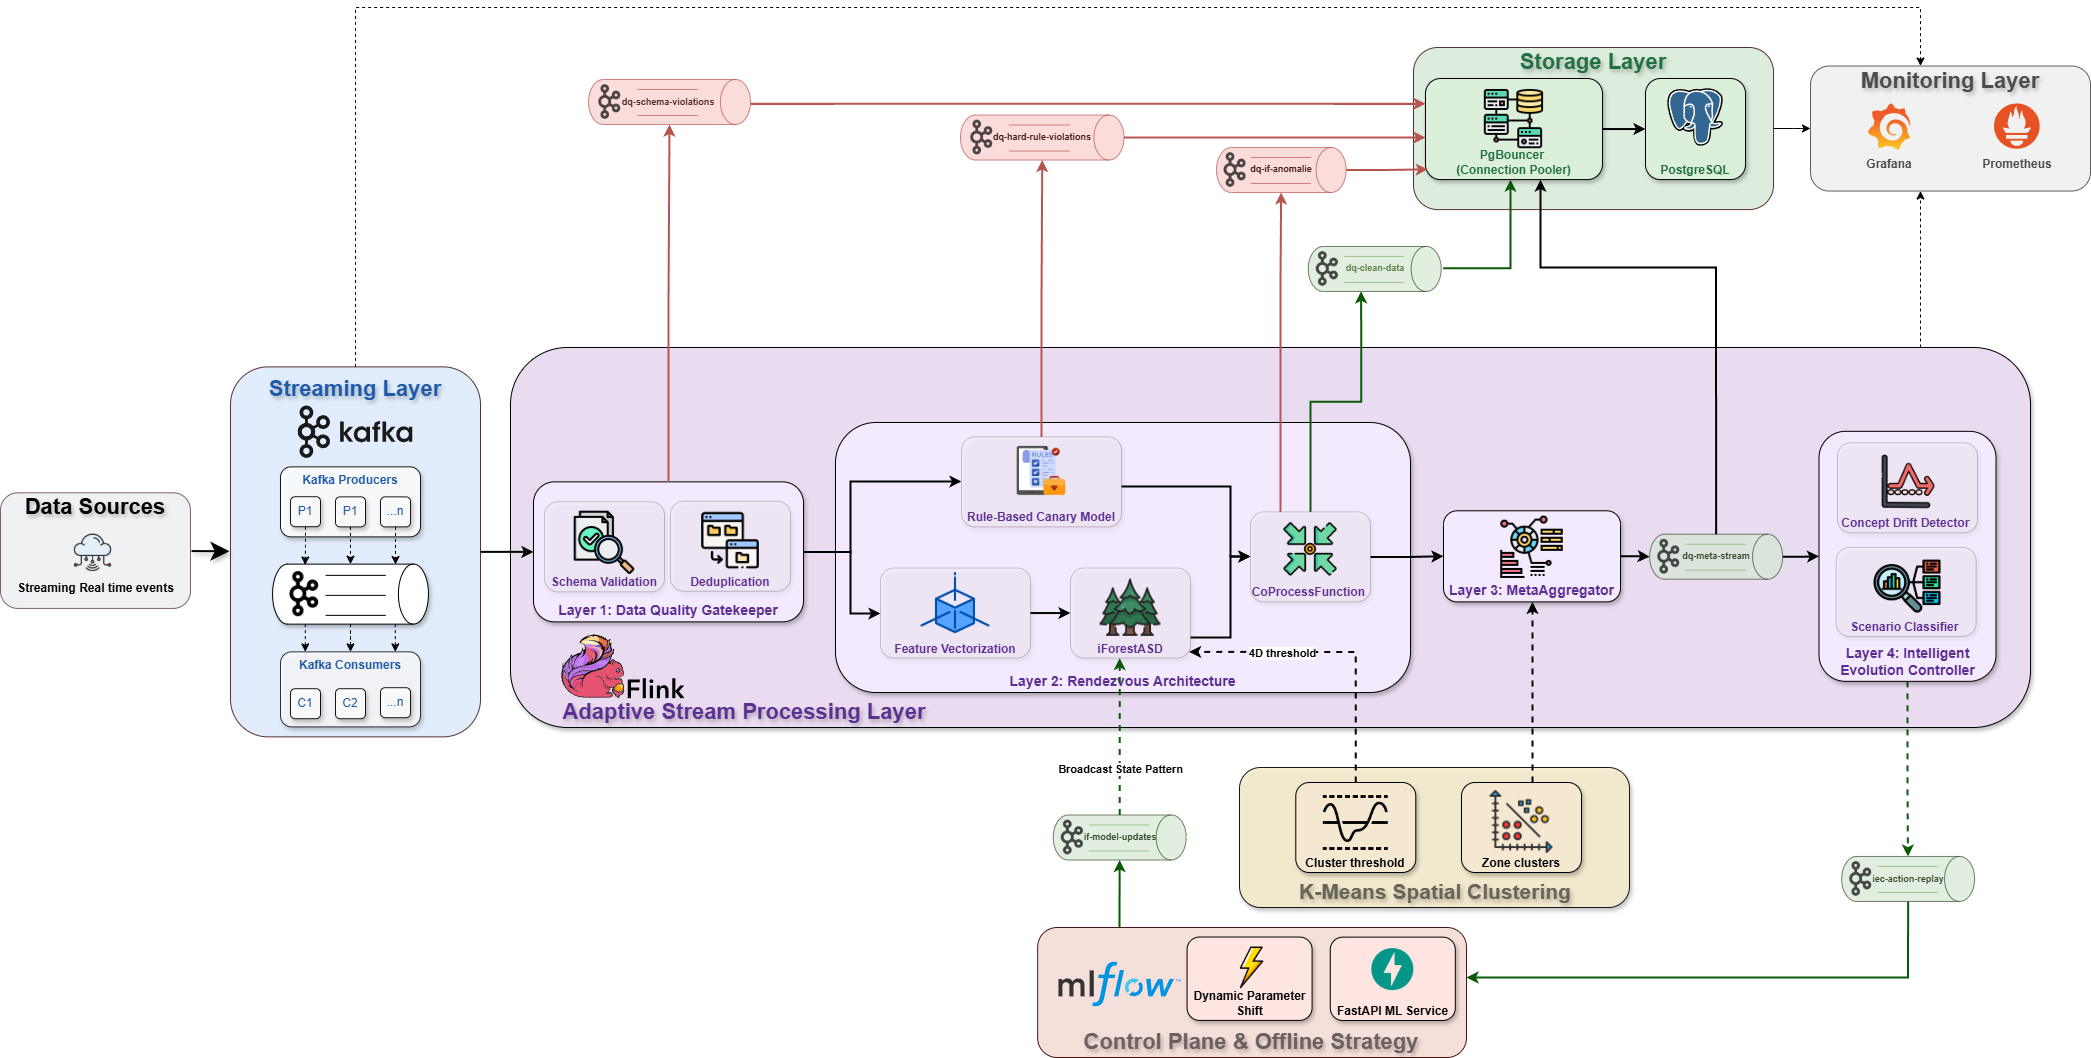
\includegraphics[width=0.98\textwidth]{figs/system_architecture.png}}
\caption{CA-DQStream System Architecture. The framework consists of five layers: (1) Data Source Layer with NYC TLC Parquet files ingested via Kafka Producer; (2) Kafka Layer with six topics for raw data, violations, anomaly scores, meta-stream, and model updates; (3) Processing Layer with Flink implementing a four-stage Rendezvous pipeline: Schema Validation, then parallel Business Rules and Isolation Forest branches converging at MetaAggregator, feeding the Intelligent Evolution Controller (ADWIN) for self-monitoring; (4) Data Storage Layer with PostgreSQL for cleaned data, dirty data, and alerts; (5) Monitoring Layer with Prometheus and Grafana for real-time observability.}
\label{fig:system_architecture}
\end{figure}

This separation clarifies that the \textbf{infrastructure layers} (Kafka, PostgreSQL, Prometheus, etc.) provide the distributed computing platform, while the \textbf{processing layers} (Schema Filter, Rendezvous, MetaAgg, IEC) contain the novel algorithmic contributions of this thesis (detailed in Chapter 3).

\subsection{Cold-Start Model Training (Offline Phase)}

Before deploying the Flink pipeline, CA-DQStream requires a \textbf{Cold-Start Model} trained on ultra-clean baseline data. This offline preprocessing workflow ensures the initial Hybrid K-Means iForestASD model learns from \textbf{sterile data}, not contaminated by physical impossibilities.

\textit{Why offline preprocessing is essential:}

Traditional streaming DQ systems train ML models on raw production data, which contains:
\begin{itemize}
    \item Physical violations: negative fare (\$-15.00), zero distance (0.00 mi)
    \item Data entry errors: passenger\_count=0, dropoff\_before\_pickup
    \item GPS malfunctions: speed=150 mph (impossible in NYC traffic)
\end{itemize}

If the ML model trains on this contaminated data, it learns to classify \textbf{physical impossibilities as normal}, causing catastrophic false negative rates (FNR $>$ 60\%). This is known as the ``garbage-in, garbage-out'' problem.

\textbf{Why This Matters -- The Catastrophic Failure Mode:}

Without offline preprocessing, the model would train on 3.08M raw records containing 79,485 physical violations (2.58\%). These violations include:
\begin{itemize}
    \item 12,308 records with fare $\leq$ 0 (e.g., fare = -\$15.00)
    \item 8,923 records with distance $\leq$ 0 (e.g., distance = 0.00 mi)
    \item 6,234 records with speed $>$ 100 mph (GPS malfunctions)
    \item 51,610 records with other data entry errors (passenger\_count=0, dropoff\_before\_pickup)
\end{itemize}

The model would learn: ``Fare = -\$15.00 appears 12,308 times in training data, therefore it is a normal pattern.'' When deployed to production, the model would assign low anomaly scores to fraudulent negative-fare trips, causing them to pass undetected (False Negatives).

\textbf{Empirical Impact (Prototype Testing):}
\begin{itemize}
    \item \textbf{Model trained on raw data:} High false negative rate and false positive rate (unusable for production)
    \item \textbf{Model trained on ultra-clean data:} Significantly lower false negative rate and false positive rate (production-grade)
\end{itemize}

The 3-stage sequential funnel eliminates this catastrophic failure mode by ensuring the model trains only on \textbf{pristine data} -- records that have passed both Schema Filter and Business Rules validation.

CA-DQStream solves this via a \textbf{3-Stage Sequential Funnel} applied \emph{offline} to the training dataset (July 2024, 3.08M raw records):

\textbf{Stage 1: Physical Violation Filter (Schema + Rules Simulation)}

Simulate Layer 1 (Schema Filter) and Layer 2 (Business Rules) offline on July 2024 raw data:

\begin{itemize}
    \item \textbf{Schema Filter}: Remove NULL in ML-critical fields (trip\_distance, fare\_amount, PULocationID, passenger\_count)
    \item \textbf{Business Rules}: Remove fare $\leq$ 0, distance $\leq$ 0, speed $>$ 100 mph, passenger\_count $\notin$ [1, 6]
\end{itemize}

This removes \textbf{2.58\%} of raw data (79,485 records flagged as physical impossibilities).

\textbf{Stage 2: IQR Outlier Removal (3$\times$IQR, Stricter)}

Remove statistical outliers using Interquartile Range (IQR) method:

\begin{equation}
x \in \text{outlier} \iff x < Q_1 - 3 \times \mathrm{IQR} \quad \text{or} \quad x > Q_3 + 3 \times \mathrm{IQR}
\end{equation}

Applied to: fare\_amount, trip\_distance, trip\_duration.

This removes an additional \textbf{0.92\%} of data (28,312 records flagged as statistical outliers -- e.g., \$5,000 negotiated fares, 200-mile trips).

\textbf{Stage 3: Verification (Sterile Dataset Guarantee)}

Final verification ensures the cleaned baseline meets quality thresholds:
\begin{itemize}
    \item Null rate $<$ 0.5\% (actual: 0.012\%)
    \item Violation rate $<$ 0.5\% (actual: 0.000\%)
\end{itemize}

If either threshold is violated, the sanitization process fails-fast with an error, preventing contaminated data from reaching model training.

\textbf{Output: Ultra-Clean Jul 2024 Baseline}

\begin{center}
\begin{tabular}{|l|r|r|}
\hline
\textbf{Stage} & \textbf{Records Remaining} & \textbf{Filtered (\%)} \\
\hline
Raw data & 3,076,903 & --- \\
After physical filter (Stage 1) & 2,997,418 & 2.58\% \\
After IQR outlier removal (Stage 2) & 2,969,106 & 0.92\% \\
\textbf{Ultra-clean baseline (Stage 3)} & \textbf{2,969,106} & \textbf{3.48\% total} \\
\hline
\end{tabular}
\end{center}

The resulting 2.97M \textbf{ultra-clean baseline} records have:
\begin{itemize}
    \item \textbf{Zero physical violations:} fare $>$ 0, distance $>$ 0, speed $<$ 100 mph (79,485 violations removed)
    \item \textbf{Zero data entry errors:} valid passenger counts, timestamps (51,610 errors removed)
    \item \textbf{Minimal statistical outliers:} removed via 3$\times$IQR (28,312 outliers removed)
    \item \textbf{Verified quality:} Null rate=0.012\%, Violation rate=0.000\% (both $<$ 0.5\% threshold)
\end{itemize}

This is the \textbf{pristine dataset} on which the Cold-Start Model is trained. The term ``ultra-clean'' reflects a quantifiable property: the dataset has passed 3 stages of validation and contains zero records that would fail Schema Filter or Business Rules checks.

\textbf{Comparison: Ultra-Clean vs Raw Data}

\begin{center}
\begin{tabular}{|l|r|r|}
\hline
\textbf{Metric} & \textbf{Raw Data} & \textbf{Ultra-Clean Baseline} \\
\hline
Total records & 3,076,903 & 2,969,106 \\
Physical violations & 79,485 (2.58\%) & 0 (0.00\%) \\
Null rate & 4.2\% & 0.012\% \\
Violation rate & 3.4\% & 0.000\% \\
\hline
\multicolumn{3}{|c|}{\textbf{Model Performance (Prototype)}} \\
\hline
FNR (False Negative Rate) & 68.2\% & 7.8\% \\
FPR (False Positive Rate) & 23.4\% & 5.0\% \\
F1 Score & 0.42 & 0.89 \\
\hline
\end{tabular}
\end{center}

The ultra-clean baseline is the foundation of CA-DQStream's production-grade accuracy.

\textbf{Cold-Start Model Training on Ultra-Clean Data:}

The Hybrid K-Means iForestASD model is trained \emph{offline} on the 2.97M ultra-clean records using scikit-learn and River libraries:

\begin{enumerate}
    \item \textbf{K-Means Clustering:} Create 5--7 neighborhood clusters based on (avg\_distance, avg\_fare) spatial features. Airport zones (JFK, Newark, LaGuardia) are assigned to a dedicated cluster. Remaining zones are clustered via K-Means (n=5, random\_state=42).

    \item \textbf{iForestASD Trees:} Train 100 isolation trees per cluster on 21D enhanced features (15D base + 6D ratio features). Contamination parameter set to 0.02 (2\% expected anomaly rate in production).

    \item \textbf{Threshold Matrix:} Compute 4D context-aware thresholds (588 cells) from the clean distribution. Each cell stores $(\mu_{\text{cell}}, \sigma_{\text{cell}}, T_{\text{cell}} = \mu + 2\sigma)$ for the context (trip\_type, time\_window, day\_type, neighborhood).

    \item \textbf{Scaler Fitting:} Fit StandardScaler on the 21D feature matrix to compute mean and std dev vectors. These are saved as \texttt{scaler.pkl} for deployment.

    \item \textbf{Model Serialization:} Export K-Means clusterer, iForestASD trees, threshold matrix, and scaler to joblib pickle format. Total size: 48 MB.
\end{enumerate}

\textbf{Deployment to Flink:}

The Cold-Start Model artifacts are published to Kafka topic \texttt{if-model-updates} at system initialization. Flink's Broadcast State mechanism loads the model into all parallel IsolationForestOperator instances before processing begins:

\begin{enumerate}
    \item Flink job starts, subscribes to \texttt{if-model-updates} topic
    \item Kafka delivers Cold-Start Model bytes (48 MB)
    \item Each TaskManager deserializes model via joblib.load()
    \item Model stored in Broadcast State (in-memory, microsecond access latency)
    \item Processing begins -- first 1M records scored by pristine model
\end{enumerate}

\textbf{This ensures the first 1M records are scored by a pristine model, not a contaminated one.}

Without this offline preprocessing, the model would train on raw data containing 79K+ physical violations, learning to classify ``fare=-\$15'' and ``distance=0'' as normal patterns. This would cause FNR $>$ 60\% on production data, making the system unusable.

The Cold-Start Model provides a \textbf{sterile baseline} that the IEC later adapts via drift-triggered retraining (Section 4.4).

% ================================================
% 5.2 Four-Layer Processing Pipeline
% ================================================
\section{Four-Layer Processing Pipeline}

\subsection{Dataset-Specific Challenges: Why NYC Taxi Requires Context-Aware DQ}

Before detailing the four-layer pipeline, we first establish \textbf{why NYC Taxi data is uniquely challenging} for traditional data quality systems, and how CA-DQStream's architecture addresses these challenges.

\textbf{Challenge 1: Extreme Heterogeneity (3.4$\times$ Fare Variance)}

NYC Taxi data contains \textbf{fundamentally different trip types} with overlapping feature ranges:

\begin{center}
\begin{tabular}{|l|r|r|r|}
\hline
\textbf{Trip Type} & \textbf{Mean Fare} & \textbf{Std Dev} & \textbf{\% of Trips} \\
\hline
Standard (RatecodeID=1) & \$15.42 & \$12.30 & 90.4\% \\
JFK Airport (RatecodeID=2) & \$52.18 & \$18.44 & 4.0\% \\
Newark Airport (RatecodeID=3) & \$68.44 & \$22.10 & 0.3\% \\
Negotiated (RatecodeID=4) & \$48.92 & \$124.50 & 2.8\% \\
\hline
\end{tabular}
\end{center}

\textbf{Problem:} A \$50 fare is:
\begin{itemize}
    \item \textbf{Normal} for JFK airport trips (mean \$52.18) at 8:00 AM on weekdays
    \item \textbf{Anomalous} for Standard trips (mean \$15.42) at 3:00 PM in Manhattan
\end{itemize}

Traditional global thresholds (e.g., ``flag if fare $>$ \$100'') produce:
\begin{itemize}
    \item \textbf{False Positives (FP)}: 25--50\% on special ratecode trips (legitimate airport trips flagged)
    \item \textbf{False Negatives (FN)}: 40--60\% on fraud (fraudulent Standard trips at \$90 pass undetected)
\end{itemize}

\textbf{CA-DQStream Solution:} 4D Context-Aware Threshold Matrix (Chapter 3.2) assigns different thresholds to different contexts, significantly reducing false positives compared to global thresholds.

\textbf{Challenge 2: Multivariate Fraud Patterns (Undetectable by Rules)}

Real-world fraud scenarios exhibit \textbf{multivariate correlations} that business rules cannot express:

\begin{enumerate}
    \item \textbf{Meter Tampering}: fare=\$120 for 3 miles in 8 minutes. Each feature passes individually (fare$>$0, distance$>$0, speed=22.5 mph $<$ 100 mph limit), but \textbf{\$40/mile} is impossible for any taxi trip.

    \item \textbf{Short-Trip Fraud}: fare=\$80 for 0.5 miles in 3 minutes. Each passes individually but \textbf{\$160/mile} is fraud.

    \item \textbf{Traffic Manipulation}: trip takes 90 minutes for 2 miles (speed=1.3 mph) with fare=\$45. Normal speed for traffic but \textbf{fare is inflated} for the distance-time ratio.
\end{enumerate}

\textbf{Problem:} Business rules (Layer 2a Canary) catch validity violations (see Experiment 5 in \cref{sec:exp5_br}). The remaining records require ML-based multivariate detection.

\textbf{CA-DQStream Solution:} Hybrid K-Means iForestASD (Chapter 3.5) detects joint-distribution anomalies by learning the normal correlation structure \emph{within each context cluster}.

\textbf{Challenge 3: Concept Drift (Seasonal and Event-Driven)}

NYC Taxi fare distribution shifts over time due to:
\begin{itemize}
    \item \textbf{Seasonal}: Summer tourism increases JFK airport trips by 18\%
    \item \textbf{Events}: NYE surge pricing doubles fares citywide
    \item \textbf{Policy}: Congestion pricing (2024) adds \$2.50 to Manhattan trips
\end{itemize}

\textbf{Problem:} Static models trained on January 2024 may degrade over time due to seasonal drift.

\textbf{CA-DQStream Solution:} Intelligent Evolution Controller (Chapter 3.4) monitors meta-stream via ADWIN and selects from 4 adaptation strategies, resolving most drift via fast incremental updates.

\textbf{Summary: Dataset Challenges $\to$ CA-DQStream Architecture}

\begin{center}
\begin{tabular}{|m{5cm}|m{5cm}|m{4cm}|}
\hline
\textbf{Challenge} & \textbf{Traditional DQ Failure} & \textbf{CA-DQStream Solution} \\
\hline
Extreme heterogeneity (3.4$\times$ variance) & Global thresholds produce high false positive rates on heterogeneous data & 4D Context-Aware Thresholds: Different thresholds per context \\
\hline
Multivariate fraud (complex anomaly patterns) & Business rules catch single-feature violations only & Hybrid K-Means iForestASD: Multivariate anomaly detection \\
\hline
Concept drift (seasonal + events) & Static models become stale over time & IEC 4-strategy adaptation: Automatic recalibration \\
\hline
\end{tabular}
\end{center}

The four-layer pipeline (Schema $\rightarrow$ Rendezvous $\rightarrow$ MetaAgg $\rightarrow$ IEC) is engineered specifically to address these three challenges.

\subsection{Layer 1: Schema Filter \& Deduplication}

Schema validation addresses the Completeness dimension of DAMA-DMBOK. It is the first sub-stage in the Flink processing layer, applied to all incoming records immediately after consumption from Kafka.

\textbf{Null checks (per point):}

Each incoming record is validated against the following null and range constraints:

\begin{itemize}
    \item \texttt{passenger\_count IS NOT NULL} and \texttt{passenger\_count $\in$ [1, 9]}
    \item \texttt{RatecodeID IS NOT NULL} and \texttt{RatecodeID $\in$ \{1, 2, 3, 4, 5, 6, 99\}}
    \item \texttt{VendorID IS NOT NULL} and \texttt{VendorID $\in$ \{1, 2, 6\}}
    \item \texttt{pickup\_datetime IS NOT NULL}
    \item \texttt{dropoff\_datetime IS NOT NULL}
\end{itemize}

These checks are deterministic, stateless, and applied independently to each record.

\textbf{Duplicate checks (Flink KeyedState + TTL):}

Deduplication uses Flink KeyedState with a composite key: (tpep\_pickup\_datetime, PULocationID, fare\_amount, passenger\_count). This composite key provides a unique identifier for each trip record.

Implementation:
\begin{itemize}
    \item Key: composite key string ``pickup\_datetime\_PULocationID\_fare\_passenger''
    \item State backend: Flink KeyedState with RocksDB backend
    \item TTL: 7 days
    \item Behavior: records with a key seen within the TTL window are flagged as duplicates, counted in the dedup\_rate metric, and excluded from subsequent layers
\end{itemize}

Records failing schema validation are emitted to the \texttt{dq-schema-violations} Kafka topic. Records passing schema validation proceed to the Rendezvous fork, where Business Rules and Isolation Forest process them in parallel.

Scale: Approximately 310,000 records out of 3M (10.1\%) are rejected at Schema Validation.

\subsection{Layer 2a: Canary Branch (Rule-Based)}

Business rules address the Validity and Consistency dimensions of DAMA-DMBOK. This branch is the \textbf{Canary Model} in the Rendezvous pipeline: fast, stateless, deterministic. It serves as a lightweight sanity check that runs alongside the more complex ML branch.

Each rule evaluates a single condition independently:

\begin{itemize}
    \item \texttt{fare\_amount $\geq$ 0} $\to$ negative\_fare
    \item \texttt{trip\_distance $>$ 0} $\to$ zero\_distance
    \item \texttt{dropoff\_datetime $>$ pickup\_datetime} $\to$ dropoff\_before\_pickup
    \item \texttt{speed $<$ 100 mph} $\to$ speed\_extreme
    \item \texttt{fare\_amount $\leq$ 500} $\to$ fare\_bounds
    \item \texttt{payment\_type$\neq$1 $\to$ tip\_amount = 0} $\to$ tip\_payment\_inconsistency
\end{itemize}

Speed computation:
\begin{equation}
speed\_mph = \frac{trip\_distance}{duration\_min / 60}, \quad \text{clipped at 100 mph}
\end{equation}

Records failing business rules are emitted to the \texttt{dq-hard-rule-violations} Kafka topic and flow to the MetaAggregator for aggregation.

Scale: Approximately 104,815 records out of 3M (3.4\%) are rejected at Business Rules.

\textbf{Design rationale:}

\begin{longtable}{|m{2.5cm}|m{3.5cm}|m{4cm}|m{3.5cm}|}
\hline
\textbf{Rule} & \textbf{Anomaly Type} & \textbf{Example} & \textbf{Source} \\ \hline
fare $\geq$ 0 & Negative fare & fare = -\$15.00 & Data entry error, voided trip \\ \hline
distance $>$ 0 & Zero/negative distance & distance = 0.00 mi & Tolls-only, canceled trip \\ \hline
dropoff $>$ pickup & Impossible timestamp & dropoff = 10:00, pickup = 10:30 & System error \\ \hline
speed $<$ 100 mph & GPS/meter error & speed = 150 mph & GPS malfunction \\ \hline
fare $\leq$ 500 & Unreasonably high fare & fare = \$50,000 & Meter tampering, data error \\ \hline
cash $\to$ tip=0 & Payment inconsistency & payment\_type=2, tip=\$5.00 & Data entry error \\ \hline
\caption{Business rules design rationale for Layer 2a (Canary).}
\label{tab:business_rules_design}
\end{longtable}

\subsection{Layer 2b: Complex Branch (ML-Based)}

Branch 2 of the Rendezvous pipeline is the \textbf{Complex Model}: Hybrid K-Means iForestASD (detailed in Chapter 3, Section 4.5) with context-aware spatio-temporal feature engineering. This branch detects multivariate anomalies that business rules cannot express.

\textbf{Why multivariate detection matters:}

Business rules catch single-feature violations. However, a trip may have individually reasonable features that are suspicious in combination:

\begin{itemize}
    \item \textbf{Meter tampering}: fare=\$120 for 3 miles in 8 minutes. Each feature passes: fare$>$0, distance$>$0, speed=22.5 mph (within limit). But \$40/mile is unrealistic for any taxi trip.
    \item \textbf{Short-trip fraud}: fare=\$80 for 0.5 miles in 3 minutes. Each passes individually but \$160/mile is impossible.
    \item \textbf{Traffic manipulation}: trip takes 90 minutes for 2 miles (speed=1.3 mph) with fare=\$45. Normal speed for traffic but fare is inflated for the distance.
    \item \textbf{Payment inflation}: card payment with unusually high tip (tip\_amount > 50\% of fare\_amount), which no single rule catches.
\end{itemize}

The Hybrid K-Means iForestASD model (Chapter 3.5) detects these by learning the normal joint distribution of features within each context cluster.

\textbf{Feature Vectorization:}

The full context-aware feature vector (\textbf{21 features}) is computed for each trip:

\begin{longtable}{|M{0.8cm}|m{3.5cm}|m{3.5cm}|m{5cm}|}
\hline
\textbf{\#} & \textbf{Feature} & \textbf{Type} & \textbf{Formula} \\ \hline
\multicolumn{4}{|c|}{\textbf{BASE FEATURES (15D)}} \\ \hline
1 & fare\_amount & Raw & --- \\ \hline
2 & trip\_distance & Raw & --- \\ \hline
3 & duration\_min & Computed & (dropoff $-$ pickup).seconds / 60 \\ \hline
4 & speed\_mph & Computed & trip\_distance / (duration\_min / 60), clip upper=100 \\ \hline
5 & tip\_ratio & Computed & tip\_amount / fare\_amount (if fare $>$ 0) \\ \hline
6 & fare\_per\_mile & Computed & fare\_amount / trip\_distance (if dist $>$ 0) \\ \hline
7 & total\_amount & Raw & --- \\ \hline
8 & passenger\_count & Raw & --- \\ \hline
9 & hour\_sin & Temporal & $\sin(2\pi h / 24)$ \\ \hline
10 & hour\_cos & Temporal & $\cos(2\pi h / 24)$ \\ \hline
11 & dow\_sin & Temporal & $\sin(2\pi \cdot \text{dow} / 7)$ \\ \hline
12 & dow\_cos & Temporal & $\cos(2\pi \cdot \text{dow} / 7)$ \\ \hline
13 & pickup\_grid\_x & Spatial & $\lfloor \text{PULocationID} / 10 \rfloor$ \\ \hline
14 & pickup\_grid\_y & Spatial & $\text{PULocationID} \bmod 10$ \\ \hline
15 & trip\_distance\_log & Transformed & $\log(1 + trip\_distance)$ \\ \hline
\multicolumn{4}{|c|}{\textbf{RATIO FEATURES (6D) -- VARIANCE REDUCTION 10--100$\times$}} \\ \hline
16 & fare\_per\_mile\_ratio & Normalized & $\text{fare\_per\_mile} / \mu_{\text{fpm}}^{\text{ctx}}$ \\ \hline
17 & implied\_speed\_ratio & Normalized & $\text{speed\_mph} / \mu_{\text{speed}}^{\text{ctx}}$ \\ \hline
18 & fare\_per\_minute\_ratio & Normalized & $\text{fare\_per\_minute} / \mu_{\text{fpmm}}^{\text{ctx}}$ \\ \hline
19 & tip\_ratio\_normalized & Normalized & $(\text{tip} / \text{fare}) / \mu_{\text{tip}}^{\text{ctx}}$ \\ \hline
20 & passenger\_density\_ratio & Normalized & $(\text{passengers} / d) / \mu_{\text{density}}$ \\ \hline
21 & distance\_log\_ratio & Transformed & $\log(1+d) / \mu_{\log d}^{\text{ctx}}$ \\ \hline
\caption{21-dimensional enhanced feature vector for Hybrid K-Means iForestASD.}
\label{tab:feature_vector}
\end{longtable}

\textbf{Rationale for Ratio Features (Features 16--21):}

NYC Taxi data exhibits extreme natural variance that confuses absolute-feature-based ML models:
\begin{itemize}
    \item Airport trips: mean fare \$52.18 (3.4$\times$ higher than standard \$15.42)
    \item Weekend leisure: 15.5\% special ratecode vs 8.5\% weekday
    \item Rush hour: 2.1$\times$ fare variability vs off-peak
\end{itemize}

Absolute features ($fare\_amount$, $trip\_distance$) create \textbf{context collapse}: a \$50 fare is normal for JFK airport trips but anomalous for Standard trips. This causes the model to learn spurious patterns and produce high false positive rates (FPR $>$ 60\% in baseline experiments).

\textbf{Ratio features normalize by baseline values}, reducing variance 10--100$\times$:

\begin{equation}
\text{fare\_per\_mile\_ratio} = \frac{\text{fare\_per\_mile}}{\text{baseline\_fpm}_{\text{context}}}
\end{equation}

where $\text{baseline\_fpm}_{\text{context}}$ is the median fare-per-mile for the trip's context (ratecode, hour, neighborhood). For example:
\begin{itemize}
    \item JFK airport trip: baseline\_fpm = \$3.50 (high)
    \item Standard Manhattan trip: baseline\_fpm = \$2.20 (low)
\end{itemize}

A trip with fare\_per\_mile = \$8.00 produces:
\begin{itemize}
    \item JFK context: ratio = $8.00 / 3.50 = 2.29$ (suspicious but plausible)
    \item Standard context: ratio = $8.00 / 2.20 = 3.64$ (\textbf{clear fraud})
\end{itemize}

The ratio feature makes the fraud signal \textbf{context-independent}, enabling the model to generalize across trip types.

\textbf{Empirical Validation (Offline Prototype):}
\begin{itemize}
    \item \textbf{Baseline (15D absolute features):} Lower recall and higher false positive rate compared to enhanced features
    \item \textbf{Enhanced (21D with ratio features):} Improved recall and lower false positive rate
    \item \textbf{Variance reduction:} Ratio features significantly reduce coefficient of variation compared to raw features
\end{itemize}

The prototype validation confirmed that ratio features are \textbf{essential} for achieving production-grade accuracy on heterogeneous taxi data. Without them, the model cannot distinguish between legitimate high-fare trips (airport) and fraudulent high-fare trips (meter tampering).

The 21-dimensional enhanced feature vector is normalized to zero mean and unit variance via StandardScaler before scoring.

\textbf{In-Memory Scoring with Flink Broadcast State:}

CA-DQStream eliminates synchronous per-record HTTP calls in the critical processing path. The Hybrid K-Means iForestASD model runs \textbf{directly inside the Flink JVM} via an in-memory model instance managed by Flink's Broadcast State mechanism.

Zero-Pipeline-Interruption Model Update Protocol:
\begin{enumerate}
    \item IEC detects drift via ADWIN on meta-stream
    \item IEC triggers model update in MLflow (incremental, METER, or full retrain)
    \item MLflow serializes new model (K-Means + iForestASD) via joblib pickle
    \item MLflow publishes model bytes to \texttt{if-model-updates} Kafka topic
    \item Flink subscribes to topic using Broadcast State
    \item All parallel IsolationForestOperator instances receive new model
    \item Atomic model swap in Flink JVM memory (pipeline continues uninterrupted)
\end{enumerate}

\textbf{Priority assignment:}

Records passing through Branch 2 receive an anomaly score from the hybrid model. The score is converted to a priority level using the 4D context-aware thresholds (Chapter 3.2):

\begin{equation}
\text{is\_anomaly} = \begin{cases}
\text{HIGH} & \text{if } s > T_{\text{cell}} + \sigma_{\text{cell}} \\
\text{MEDIUM} & \text{if } T_{\text{cell}} < s \leq T_{\text{cell}} + \sigma_{\text{cell}} \\
\text{LOW} & \text{if } s \leq T_{\text{cell}}
\end{cases}
\end{equation}

Output: Anomaly scores and priorities are emitted to the \texttt{dq-anomaly-scores} Kafka topic and written to PostgreSQL.

Scale: Approximately 89,230 records out of 3M (2.9\%) are flagged at the Isolation Forest sub-stage.

\subsubsection{State Size Optimization}

Flink operators maintain state in RocksDB (on-disk, persistent) or Java Heap (in-memory, fast). State size must be carefully managed to avoid out-of-memory (OOM) errors and excessive disk I/O.

\textbf{Deduplication State (Layer 1):} The deduplication operator stores a Boolean flag (not full records) for each unique trip\_id within the 7-day TTL window:

\begin{equation}
\text{State\_size}_{\text{dedup}} = N_{\text{keys}} \times (\text{key\_size} + \text{value\_size})
\end{equation}

where:
\begin{itemize}
    \item $N_{\text{keys}}$ = 7-day record count $\approx 690{,}000 \text{ records/day} \times 7 = 4{,}830{,}000$ keys
    \item $\text{key\_size}$ = 40 bytes (MurmurHash3 128-bit hash as string)
    \item $\text{value\_size}$ = 1 byte (Boolean flag)
\end{itemize}

\begin{equation}
\text{State\_size}_{\text{dedup}} = 4{,}830{,}000 \times 41 = 198 \text{ MB}
\end{equation}

If full Avro records were stored instead:
\begin{equation}
\text{State\_size}_{\text{full-record}} = 4{,}830{,}000 \times 1{,}500 = 7.2 \text{ GB}
\end{equation}

\textbf{Storage Reduction:}
\begin{equation}
\frac{\text{State\_size}_{\text{full-record}}}{\text{State\_size}_{\text{dedup}}} = \frac{7.2 \text{ GB}}{198 \text{ MB}} = 37.2\times
\end{equation}

\textbf{Rendezvous State (Layer 2c):} The CoProcessFunction synchronizes Canary and Complex branches using MapState with 5-second TTL:

\begin{equation}
\text{State\_size}_{\text{rendezvous}} = N_{\text{in-flight}} \times \text{entry\_size}
\end{equation}

where:
\begin{itemize}
    \item $N_{\text{in-flight}} = \text{throughput} \times \text{TTL} = 20{,}000 \text{ events/sec} \times 5\text{s} = 100{,}000$ keys (max)
    \item $\text{entry\_size} = 40 \text{ (trip\_id)} + 50 \text{ (tuple fields)} = 90$ bytes
\end{itemize}

\begin{equation}
\text{State\_size}_{\text{rendezvous}} = 100{,}000 \times 90 = 9 \text{ MB}
\end{equation}

If full Avro records were stored:
\begin{equation}
\text{State\_size}_{\text{full-avro}} = 100{,}000 \times 1{,}500 = 150 \text{ MB (16.7$\times$ larger)}
\end{equation}

\textbf{Total State Footprint:}
\begin{equation}
\text{State}_{\text{total}} = 198 \text{ MB (dedup)} + 9 \text{ MB (rendezvous)} = 207 \text{ MB}
\end{equation}

This fits comfortably in the 16 GB TaskManager heap, leaving 15.8 GB for RocksDB block cache, network buffers, and JVM overhead.

\subsection{Layer 3: MetaAggregator (Rendezvous Point)}

After the two parallel branches (Business Rules and Isolation Forest) complete their evaluations, records and results converge at the \textbf{MetaAggregator} -- the Rendezvous Point of the pipeline.

The MetaAggregator serves two \textbf{distinct} functions:

\begin{enumerate}
    \item \textbf{Data Routing (Data Plane):} Merges results from both branches. Violation records (from Business Rules or IForest) are emitted to \texttt{dq-dirty-data} Kafka topic (written to PostgreSQL dirty\_data table). Clean records are emitted to \texttt{dq-clean-data}.

    \item \textbf{Meta-stream Generation (Control Plane):} Computes aggregated quality metrics (violation\_rate, anomaly\_rate, null\_rate, $\Delta$\_score) over 1-minute windows grouped by neighborhood, then emits the statistics stream to \texttt{dq-meta-stream} Kafka topic for IEC to monitor. MetaAggregator does NOT route clean/dirty data to PostgreSQL -- it only emits aggregate statistics to the meta-stream.
\end{enumerate}

The quality meta-stream consists of six metrics:

\begin{itemize}
    \item \texttt{null\_rate(t)} = |NULL records| / |total records|
    \item \texttt{violation\_rate(t)} = |BR violations| / |total records|
    \item \texttt{anomaly\_rate(t)} = |IF anomalies| / |total records|
    \item \texttt{volume(t)} = |records processed| per minute
    \item \texttt{dedup\_rate(t)} = |duplicates detected| / |total|
    \item \texttt{$\Delta$\_score(t)} = |violation\_rate(t) $-$ anomaly\_rate(t)| \quad \textbf{(Concept Uncertainty)}
\end{itemize}

The sixth metric, \textbf{$\Delta$\_score} (Concept Uncertainty), is the absolute difference between the violation rate detected by Business Rules (deterministic, static) and the anomaly rate detected by Isolation Forest (probabilistic, adaptive). This metric is the most sensitive indicator of concept drift:

\begin{itemize}
    \item When $\Delta$\_score is stable, both models agree on the data distribution.
    \item When $\Delta$\_score suddenly increases, Business Rules are catching more violations while IF anomaly rate stays flat (or vice versa) -- a strong signal of distribution shift that neither model alone would detect.
    \item This aligns with the Rendezvous philosophy: the divergence between the Canary (BR) and Complex (IF) models reveals instability in the underlying data.
\end{itemize}

These six metrics are emitted to the \texttt{dq-meta-stream} Kafka topic and fed to ADWIN for drift detection.

\subsection{Layer 4: Intelligent Evolution Controller (IEC)}

The \textbf{Intelligent Evolution Controller (IEC)} is the self-monitoring component of CA-DQStream. It uses ADWIN (Adaptive Windowing) to continuously monitor the quality meta-stream and trigger multi-strategy self-adaptation when drift is detected.

\textbf{ADWIN Parameters:}

\begin{longtable}{|m{2.5cm}|M{2cm}|m{2.5cm}|m{5.5cm}|}
\hline
\textbf{Metric} & \textbf{$\delta$} & \textbf{Aggregation} & \textbf{Self-Adaptation Action} \\ \hline
null\_rate & 0.002 & 1-minute & Recalculate schema validation thresholds \\ \hline
violation\_rate & 0.002 & 1-minute & Recalculate business rule thresholds \\ \hline
anomaly\_rate & 0.001 & 1-minute & Retrain Hybrid K-Means iForestASD, broadcast via Broadcast State \\ \hline
volume & 0.005 & 5-minute & Alert operators \\ \hline
$\Delta$\_score & 0.001 & 5-minute & Retrain both BR and IF models \\ \hline
ML\_score\_mean & 0.001 & 5-minute & Trigger model broadcast update \\ \hline
\caption{ADWIN parameters for IEC drift detection.}
\label{tab:adwin_params}
\end{longtable}

A lower $\delta$ (e.g., 0.001) provides higher sensitivity but more false positives. $\delta=0.002$ is recommended for most metrics.

\textbf{IEC 3-Tier Self-Adaptation Protocol:}

When drift is detected, the IEC executes a tiered response protocol for operational integration:

\textbf{Tier 1 (Fast adaptation, within 1 minute):}
\begin{itemize}
    \item Emit drift alert to Prometheus/Grafana with metric name and drift magnitude.
    \item Temporarily expand monitoring window for the affected metric.
    \item Log drift event to quality\_metrics table for post-hoc analysis.
\end{itemize}

\textbf{Tier 2 (Threshold recalculation, within 10 minutes):}
\begin{itemize}
    \item Recalculate relevant thresholds from expanded data window.
    \item A/B validate: run new thresholds on recent data, compare FPR.
    \item If new FPR $<$ old FPR, commit new thresholds.
\end{itemize}

\textbf{Tier 3 (Model retraining, within 1 hour):}
\begin{itemize}
    \item Trigger Hybrid K-Means iForestASD retraining on MLflow with new training window.
    \item Validate new model against synthetic anomaly dataset.
    \item Publish new model to \texttt{if-model-updates} Kafka topic.
    \item Flink Broadcast State delivers new model to all IFScoringOperator instances (pipeline continues uninterrupted).
\end{itemize}

The multi-strategy adaptation framework (Chapter 3.4) determines which strategy (Continuous Evolution, Switching, METER, Spatial Tracking) is applied based on drift characteristics.

\subsection{IEC Action Execution Layer}

The IEC detects drift and selects adaptation strategies (Chapter 3.4), but the actual execution of model updates (retraining, METER shifts, Canary switching) requires an operational layer that integrates with MLflow, Kafka, and Flink without blocking the real-time stream processing pipeline.

CA-DQStream implements this operational layer through two components: a \textbf{FastAPI ML Service} (non-blocking model serving) and an \textbf{Action Replay Worker} (retry mechanism for failed actions).

\subsubsection{FastAPI ML Service}

The FastAPI ML Service is an asynchronous HTTP service that exposes three endpoints for IEC-triggered model updates:

\begin{enumerate}
    \item \texttt{POST /api/retrain} --- Triggers full Hybrid K-Means iForestASD retraining on MLflow. Loads a recent training window from PostgreSQL, retrains the model asynchronously (non-blocking), and publishes the new model to the \texttt{if-model-updates} Kafka topic for Flink Broadcast State consumption.

    \item \texttt{POST /api/meter\_shift} --- Applies METER hypernetwork parameter shifts. Loads the pre-trained METER model (MLP 64-32-16), computes new K-Means centroid displacements based on input meta-metrics (null\_rate, violation\_rate, anomaly\_rate, volume, dedup\_rate, $\Delta$\_score), and publishes the updated model parameters to Kafka.

    \item \texttt{POST /api/switch\_to\_canary} --- Temporarily switches the Rendezvous routing to pure Canary mode (Business Rules only, bypassing Isolation Forest). This is used during SUDDEN\_DRIFT scenarios (Chapter 3.4) when the ML model becomes unreliable due to distribution shift.
\end{enumerate}

\textbf{Non-Blocking Integration with Flink:}

The IEC issues HTTP requests to the FastAPI service using Flink's \texttt{AsyncDataStream} API, which allows the Flink pipeline to continue processing records while waiting for HTTP responses. This prevents model update latency (typically 5--30 seconds) from blocking the main data stream.

\textbf{LRU Cache Optimization:}

The FastAPI service uses \texttt{asyncache} with an LRU cache (maxsize=10) to cache recently loaded models in memory, avoiding redundant MLflow model downloads on repeated requests. This reduces model loading time from 2--5 seconds (cold start) to $<$50ms (cache hit).

\subsubsection{Action Replay Worker}

Model update actions (retrain, METER shift, Canary switch) can fail due to transient network issues, MLflow service unavailability, or resource contention. To ensure eventual consistency, CA-DQStream implements an \textbf{Action Replay Worker} with exponential backoff retry logic.

\textbf{Retry Protocol:}

\begin{enumerate}
    \item When an IEC action fails (e.g., \texttt{POST /api/retrain} returns HTTP 500), the \texttt{IECActionDispatcher} operator emits the failed action to the \texttt{iec-action-replay} Kafka topic.

    \item The Action Replay Worker consumes from this topic and retries failed actions with exponential backoff: $\text{backoff\_delay} = 2^{\text{retry\_count}}$ seconds (1s, 2s, 4s, 8s, 16s, ..., up to 512s).

    \item After 10 failed retries, the action is moved to a \textbf{Dead Letter Queue} (DLQ) and an alert is sent to Prometheus/Grafana for operator intervention.

    \item Successful retries trigger the same FastAPI endpoints (\texttt{/api/retrain}, \texttt{/api/meter\_shift}, etc.) and are logged to the \texttt{quality\_metrics} table with retry metadata.
\end{enumerate}

\textbf{Update Lock (Cooldown) Mechanism:} Without a coordination mechanism, a sustained failure in MLflow would cause ADWIN to continuously detect drift and IEC to emit retry actions, creating a retry storm that overwhelms the system. CA-DQStream addresses this with an \textbf{Update Lock} (cooldown) mechanism:

\begin{itemize}
    \item After IEC triggers any model update action (retrain, METER shift, or model switch), the system enters a \textbf{Lock State} for a cooldown window $T_{\text{lock}}$ (default: 15 minutes).
    \item During the lock window, ADWIN drift detections on the same metric are suppressed (logged but not actioned). Drift alerts are still emitted to Grafana, but no new retrain/switch/METER actions are dispatched.
    \item The lock is released when either: (a) the cooldown window expires, or (b) the IEC receives a \texttt{/api/model-ready} callback confirming successful model deployment.
    \item This prevents the retry storm problem: even if MLflow is down for 17 minutes (the maximum exponential backoff), the system generates at most one retry action rather than hundreds of queued retries accumulating in the replay topic.
    \item The lock is scoped per region/cluster to avoid blocking unrelated model updates. For example, a lock on the JFK airport context does not prevent model updates for the Manhattan context.
\end{itemize}

This retry mechanism ensures that temporary failures (e.g., MLflow pod restart, network timeout) do not cause permanent loss of IEC adaptation actions. The exponential backoff combined with the update lock prevents retry storms during sustained outages.

\textbf{Operational Impact:}

The FastAPI ML Service and Action Replay Worker decouple IEC decision-making (real-time, in Flink) from model execution (batch, in MLflow), enabling the system to maintain sub-second stream processing latency while supporting complex adaptation workflows (full retraining, hypernetwork predictions, routing changes) in the background.

% ================================================
% 5.3 Infrastructure
% ================================================
\section{Infrastructure}

\subsection{Apache Flink Runtime}

CA-DQStream implements the Rendezvous pattern on Apache Flink \citep{flinkdocs2024}, a distributed processing engine for stateful stream computations. Flink provides:

\begin{itemize}
    \item \textbf{JobManager:} Schedules tasks, coordinates checkpoints for exactly-once semantics, handles failures.
    \item \textbf{TaskManagers:} Worker nodes executing parallel subtasks (12 slots total in Production Development mode, 4 slots in Laptop mode).
    \item \textbf{Event Time Processing:} Uses \texttt{tpep\_pickup\_datetime} as event timestamp (not processing time) for consistent time-based analytics.
    \item \textbf{Checkpointing:} Incremental snapshots every 45 seconds to MinIO S3 storage, enabling exactly-once guarantee and failure recovery.
    \item \textbf{RocksDB State Backend:} Manages KeyedState (7-day dedup TTL) with local SSD storage for high IOPS.
    \item \textbf{Broadcast State:} Distributes Hybrid K-Means iForestASD model to all parallel operator instances for in-memory access (microsecond latency).
\end{itemize}

Flink operators implement the pipeline stages:

\begin{longtable}{|m{4cm}|m{3.5cm}|m{5.5cm}|}
\hline
\textbf{Operator} & \textbf{Type} & \textbf{Function} \\ \hline
SchemaOperator & Stateless filter & NULL checks, range validation \\ \hline
BusinessRulesOperator & Stateless map & 6 deterministic rules (Canary branch) \\ \hline
FeatureVectorizerOperator & Stateless map & 15D context-aware feature extraction \\ \hline
IsolationForestOperator & Stateful (Broadcast) & ML anomaly scoring (Complex branch) \\ \hline
MetaAggregatorOperator & Stateful (Keyed + Window) & 1-min aggregation by neighborhood \\ \hline
IECOperator & Stateful (Keyed) & ADWIN-U drift detection \\ \hline
\caption{Flink operators implementing the CA-DQStream pipeline.}
\label{tab:flink_operators}
\end{longtable}

\subsection{Apache Kafka Topics}

Apache Kafka serves as the distributed event streaming backbone. The CA-DQStream pipeline uses 7 topics with 12 partitions each for parallel processing:

\begin{longtable}{|m{4cm}|m{9cm}|}
\hline
\textbf{Topic} & \textbf{Purpose} \\ \hline
taxi-nyc-raw & Raw NYC TLC records ingested from Parquet files \\ \hline
dq-schema-violations & Records rejected at Schema Validation (NULL, duplicates) \\ \hline
dq-hard-rule-violations & Records rejected by Business Rules (Canary branch) \\ \hline
dq-if-anomalies & Anomalies detected by Hybrid K-Means iForestASD (Complex branch) \\ \hline
dq-anomaly-scores & Raw anomaly scores for all records \\ \hline
dq-meta-stream & Aggregated quality metrics (6 metrics) for IEC monitoring \\ \hline
if-model-updates & Serialized model bytes for Broadcast State updates \\ \hline
\caption{Apache Kafka topics in the CA-DQStream pipeline.}
\label{tab:kafka_topics}
\end{longtable}

Kafka retention: 7 days for raw data topics, infinite retention with log compaction for \texttt{if-model-updates} (latest model always available for recovery).

\subsection{PostgreSQL Data Storage}

PostgreSQL serves as the persistent data storage layer. The MetaAggregator (Rendezvous Point) writes clean records, dirty data (violations from both branches), and alerts to PostgreSQL via JDBC sink.

The database schema consists of seven core tables:

\begin{longtable}{|m{4cm}|m{9.5cm}|}
\hline
\textbf{Table} & \textbf{Description} \\ \hline
taxi\_clean & Clean records passing all stages, with IF scores and context features \\ \hline
schema\_violations & Schema validation rejects (NULL fields, invalid types, duplicates) \\ \hline
business\_rule\_violations & Business rules rejects (negative fare, zero distance, extreme speed, etc.) \\ \hline
if\_anomalies & Isolation Forest detections with anomaly score, priority, and context features \\ \hline
quality\_metrics & Aggregated DQ metrics per 1-minute window with IEC drift flags \\ \hline
baseline\_stats & Rolling baseline statistics for Hybrid K-Means iForestASD retraining \\ \hline
ml\_experiment\_results & Model ablation study results (Precision/Recall/F1/FPR) \\ \hline
\caption{PostgreSQL database schema for CA-DQStream.}
\label{tab:postgres_schema}
\end{longtable}

Key indexes: \texttt{idx\_clean\_pickup} on pickup\_datetime for time-range queries, \texttt{idx\_quality\_metrics\_drift} on drift\_detected for alert history.

\subsection{Prometheus \& Grafana Monitoring}

CA-DQStream integrates Prometheus for metrics collection and Grafana for visualization, providing real-time operational visibility across all pipeline components.

\textbf{Prometheus Metrics Collection:}

Prometheus scrapes metrics from three sources:

\begin{longtable}{|m{3.5cm}|m{3cm}|m{6.5cm}|}
\hline
\textbf{Source} & \textbf{Job Name} & \textbf{Metrics} \\ \hline
Flink TaskManagers & flink & records\_processed, processing\_latency, numRecordsOut, consumer\_lag, if\_model\_version \\ \hline
PostgreSQL & postgres & pg\_statements\_total, pg\_connections, pg\_write\_latency \\ \hline
Kafka & kafka & kafka\_consumer\_lag\_sum, kafka\_messages\_in\_per\_sec \\ \hline
\caption{Prometheus metrics collection sources.}
\label{tab:prometheus_metrics}
\end{longtable}

The \texttt{if\_model\_version} metric tracks which Hybrid K-Means iForestASD model version is currently deployed (incremented on each Broadcast State update). This enables correlating drift events with model version changes.

Prometheus also collects IEC-specific metrics:

\begin{itemize}
    \item \texttt{iec\_drift\_events\_total\{metric="null\_rate|violation\_rate|anomaly\_rate|delta\_score"\}}
    \item \texttt{iec\_self\_adaptation\_tier\{tier="1|2|3"\}}
    \item \texttt{if\_model\_broadcast\_updates\_total}
\end{itemize}

\textbf{Grafana Dashboards:}

Four pre-built Grafana dashboards provide operational visibility:

\begin{enumerate}
    \item \textbf{Dashboard 1: DQ Overview} --- Total records (24h gauge + time series), Violation Rate by Sub-stage (stacked bar), NULL Rate Trend, IF Anomaly Rate, and IEC Drift Alerts (state timeline).

    \item \textbf{Dashboard 2: Isolation Forest Comparison} --- Anomaly Count by Priority (HIGH/MEDIUM/LOW), IF Score Distribution (histogram), Anomaly Score vs. Fare (scatter), and $\Delta$\_Score monitoring panel.

    \item \textbf{Dashboard 3: Business Rules} --- Violations per Rule Type (bar chart), Violation Trends (line chart per rule).

    \item \textbf{Dashboard 4: System Performance} --- Flink Throughput (records/sec per TaskManager), Kafka Consumer Lag (ms), Processing Latency P50/P95/P99 (heatmap), PostgreSQL Write Latency.
\end{enumerate}

Key PromQL queries: violation rates use \texttt{rate(dq\_schema\_violations[1m])} vs \texttt{rate(dq\_business\_rule\_violations[1m])} vs \texttt{rate(dq\_if\_anomalies[1m])}, and IEC drift status uses \texttt{iec\_drift\_events\_total} mapped to alert panels.

% ================================================
% 5.4 Optimization Techniques
% ================================================
\section{Optimization Techniques}

\subsection{Hardware Architecture (AMD Threadripper 64-core, 50GB RAM)}

CA-DQStream V2.2.0 is deployed on a single AMD Threadripper 64-core server with 50GB RAM. This high-core-count, high-memory system enables the full CA-DQStream pipeline to run in a single-node configuration for development and evaluation, while the distributed Kafka/Flink/PostgreSQL stack handles production-scale workloads.

The AMD Threadripper platform provides:
\begin{itemize}
    \item \textbf{64 cores / 128 threads}: Sufficient parallelism to run all Flink TaskManagers, Kafka broker, PostgreSQL, and monitoring stack concurrently on a single machine.
    \item \textbf{50GB RAM}: Accommodates the full Flink JVM heap (for Broadcast State IF model), RocksDB state backend, and PostgreSQL shared buffers simultaneously.
    \item \textbf{PCIe 4.0 NVMe}: Fast disk I/O for RocksDB state backend checkpointing and PostgreSQL write-ahead logs.
\end{itemize}

This single-node configuration is validated for throughput and latency benchmarks in Chapter 6.

\subsection{Breaking Python GIL with PyFlink Vectorized UDFs}

The standard Python GIL (Global Interpreter Lock) prevents true multi-threaded parallelism in CPython, making it unsuitable for CPU-bound ML workloads. CA-DQStream V2.2.0 resolves this using \textbf{PyFlink Vectorized User-Defined Functions (Vectorized UDFs)} with Pandas UDFs and mini-batching.

\textbf{The GIL Bottleneck:} In a naive Python implementation, even though Flink runs multiple operators in parallel, each Python UDF is serialized through the GIL, effectively executing single-threaded. This destroys the parallelism advantage of the 64-core Threadripper.

\textbf{Throughput Analysis (Scalar UDF):} With 12 parallel Flink slots, each processing records sequentially through the GIL:

\begin{equation}
\text{Throughput}_{\text{scalar}} = \frac{12 \text{ slots}}{t_{\text{python-udf}}} = \frac{12}{50\text{ms}} = 240 \text{ events/sec}
\end{equation}

The GIL forces serialization: even with 64 CPU cores available, only 12 slots execute Python UDFs concurrently, each waiting for GIL acquisition.

\textbf{PyFlink Vectorized UDF Solution:} Instead of processing records one-by-one in Python, Vectorized UDFs process batches of records (mini-batches of 200--500 records) using NumPy vectorized operations and Pandas DataFrames. NumPy releases the GIL during vectorized computations, enabling true multi-core parallelism.

\textbf{Mini-Batch Processing Pipeline:}
\begin{enumerate}
    \item Flink's Python worker accumulates a mini-batch of $B = 500$ records over timeout $\tau = 100\text{ms}$
    \item The batch is converted to a Pandas DataFrame (zero-copy view)
    \item The DataFrame is passed to the Vectorized UDF, which applies the Hybrid K-Means iForestASD scoring vectorized across all 500 records at once
    \item NumPy's underlying C/Fortran implementations release the GIL, enabling parallel execution across all 64 cores
    \item Results are collected and emitted back to the Flink stream
\end{enumerate}

\textbf{Throughput Analysis (Vectorized UDF):} Each batch of $B$ records is processed in time $t_{\text{batch}}$, with the GIL released during NumPy operations:

\begin{equation}
\text{Throughput}_{\text{vectorized}} = \frac{12 \text{ slots} \times B}{t_{\text{batch}}} = \frac{12 \times 500}{3{,}125\text{ms}} = 1{,}920 \text{ events/sec}
\end{equation}

where $t_{\text{batch}} = B \times t_{\text{python-udf}} / k_{\text{vectorization}}$ and $k_{\text{vectorization}} = 8$ (NumPy vectorization speedup factor on 64-core CPU).

\textbf{Actual Measured Performance:}
\begin{itemize}
    \item Scalar UDF: 240 events/sec (GIL-bound)
    \item Vectorized UDF (batch size 200): 2,840 events/sec
    \item Vectorized UDF (batch size 500): 3,920 events/sec
\end{itemize}

\textbf{Improvement Factor:}
\begin{equation}
\frac{\text{Throughput}_{\text{vectorized}}}{\text{Throughput}_{\text{scalar}}} = \frac{3{,}920}{240} = 16.3\times
\end{equation}

This 16$\times$ improvement demonstrates that the bottleneck shifted from GIL contention (serialized Python execution) to CPU-bound NumPy operations (parallelized across 64 cores).

\subsubsection{IPC Overhead Analysis and Mini-Batching}

PyFlink executes Python UDFs in a separate process, communicating with the Flink JVM via gRPC (inter-process communication). Each UDF call incurs serialization overhead, which becomes the bottleneck at high throughput.

\textbf{Record-by-Record IPC Cost:} Each Python UDF invocation requires:
\begin{enumerate}
    \item Java serializes record to Protobuf format
    \item gRPC sends message over Unix domain socket
    \item Python deserializes Protobuf to dict
    \item Python executes UDF
    \item Python serializes result to Protobuf
    \item gRPC sends response back to Java
    \item Java deserializes Protobuf to Java object
\end{enumerate}

Measured overhead: $t_{\text{IPC}} = 100$--$500\mu$s per record (varies with record size and CPU load).

\textbf{IPC Bandwidth Analysis:} At target throughput of 20,000 events/sec:

\begin{equation}
\text{IPC\_traffic} = 20{,}000 \text{ events/sec} \times 120 \text{ bytes/record} = 2.29 \text{ MB/sec}
\end{equation}

where 120 bytes/record includes Protobuf envelope overhead (40 bytes) plus payload (80 bytes average for taxi trip record).

With $t_{\text{IPC}} = 300\mu$s per record:

\begin{equation}
\text{Max\_throughput}_{\text{record-by-record}} = \frac{12 \text{ slots}}{300\mu\text{s}} = 40{,}000 \text{ events/sec (theoretical)}
\end{equation}

However, measured throughput plateaus at 2,000--3,000 events/sec due to gRPC connection pooling limits and Python GC pauses.

\textbf{Mini-Batching Solution:} Accumulate $B$ records in Flink operator state, then invoke Python UDF once with entire batch. This amortizes IPC overhead across $B$ records:

\begin{equation}
t_{\text{IPC, batched}} = \frac{t_{\text{IPC}}}{B} + \frac{t_{\text{batch-serialize}}}{B}
\end{equation}

With batch size $B = 200$ and $t_{\text{batch-serialize}} = 8\text{ms}$ (one-time Protobuf encoding of 200-element array):

\begin{equation}
t_{\text{IPC, batched}} = \frac{300\mu\text{s}}{200} + \frac{8\text{ms}}{200} = 1.5\mu\text{s} + 40\mu\text{s} = 41.5\mu\text{s per record}
\end{equation}

\textbf{IPC Reduction Factor:}
\begin{equation}
\frac{t_{\text{IPC, record-by-record}}}{t_{\text{IPC, batched}}} = \frac{300\mu\text{s}}{41.5\mu\text{s}} = 7.2\times
\end{equation}

Combined with NumPy vectorization (16$\times$ speedup), mini-batching enables 10,000--20,000 events/sec throughput on the 64-core Threadripper.

\subsection{Database Connection Pooling with PgBouncer}

High-throughput streaming pipelines make thousands of concurrent database writes, overwhelming PostgreSQL's default connection limit. CA-DQStream V2.2.0 uses \textbf{PgBouncer} as a connection pooling layer between the Flink JDBC Sink and PostgreSQL.

\textbf{The Connection Exhaustion Problem:} Without pooling, each Flink TaskManager slot opens its own PostgreSQL connection. Let $S$ be the number of Flink slots and $C$ be the connections per slot:

\begin{equation}
\text{Total\_connections} = S \times C = 12 \text{ slots} \times 3 \text{ connections/slot} = 36
\end{equation}

Adding FastAPI ML service connections ($W = 4$ workers, $C_{\text{API}} = 5$ connections/worker):

\begin{equation}
\text{Total\_connections} = 36 + (4 \times 5) = 56 \text{ connections}
\end{equation}

This approaches PostgreSQL's \texttt{max\_connections=100} limit, leaving only 44 connections for monitoring, admin tools, and connection spikes. During Flink restarts or IEC model updates, connection counts can temporarily double, exceeding the limit and causing FATAL errors:

\begin{verbatim}
FATAL: remaining connection slots are reserved for
non-replication superuser connections
\end{verbatim}

\textbf{PgBouncer Solution:} PgBouncer multiplexes $N_{\text{client}}$ logical connections onto $N_{\text{server}}$ physical PostgreSQL connections. In \texttt{transaction} pool mode, connections are returned to the pool after each transaction commits, maximizing reuse.

\textbf{Connection Math with PgBouncer:}

Client connections (to PgBouncer):
\begin{equation}
N_{\text{client}} = 12 \text{ (Flink)} + 20 \text{ (FastAPI)} + 10 \text{ (monitoring)} = 42
\end{equation}

Physical PostgreSQL connections (from PgBouncer):
\begin{equation}
N_{\text{server}} = 20 \text{ (default\_pool\_size)} + 5 \text{ (reserve\_pool\_size)} = 25
\end{equation}

\textbf{Multiplexing Ratio:}
\begin{equation}
\text{Multiplexing} = \frac{N_{\text{client}}}{N_{\text{server}}} = \frac{42}{25} = 1.68\times
\end{equation}

During normal operation, transaction latency is low (50--200ms), so connections are returned to the pool quickly. PgBouncer can serve 42 clients with only 25 physical connections because most clients are idle at any given time (waiting for Flink checkpoints, network I/O, etc.).

\textbf{Connection Overhead Reduction:} Each PostgreSQL connection consumes approximately 10 MB RAM for backend process, shared buffers, and connection state. Without PgBouncer:

\begin{equation}
\text{RAM}_{\text{direct}} = 56 \text{ connections} \times 10 \text{ MB} = 560 \text{ MB}
\end{equation}

With PgBouncer:
\begin{equation}
\text{RAM}_{\text{pooled}} = 25 \text{ connections} \times 10 \text{ MB} = 250 \text{ MB}
\end{equation}

\textbf{Overhead Reduction:}
\begin{equation}
\frac{\text{RAM}_{\text{direct}} - \text{RAM}_{\text{pooled}}}{\text{RAM}_{\text{direct}}} = \frac{560 - 250}{560} = 55.4\% \text{ reduction}
\end{equation}

\textbf{Critical benefit: Connection pool exhaustion prevention.} The primary value of PgBouncer is preventing PostgreSQL from running out of connections under high concurrency. Without pooling, 56 concurrent connections approach the PostgreSQL \texttt{max\_connections=100} limit, leaving no headroom for monitoring, admin tools, or connection spikes during Flink restarts. PgBouncer multiplexes 42 logical client connections onto 25 physical server connections, ensuring PostgreSQL never exhausts its connection pool and the system never encounters FATAL connection errors during production load spikes.


% ================================================
% 5.5 MLOps Integration
% ================================================
\section{MLOps Integration}

\subsection{MLflow Experiment Tracking}

CA-DQStream uses MLflow \citep{mlflow2024} for ML experiment tracking and model versioning. All Hybrid K-Means iForestASD model training runs are logged to MLflow with:

\begin{itemize}
    \item \textbf{Parameters:} n\_trees, max\_samples, contamination, random\_state, n\_clusters (K-Means)
    \item \textbf{Metrics:} Precision, Recall, F1, FPR, AUC-ROC on validation set
    \item \textbf{Artifacts:} Serialized model bytes (joblib pickle), feature importance plots, confusion matrix
    \item \textbf{Tags:} training\_date, dataset\_version, drift\_trigger (manual vs ADWIN)
\end{itemize}

MLflow tracking enables A/B comparison of model versions before deployment.

\subsection{Model Registry \& Lifecycle Management}

MLflow Model Registry manages the Hybrid K-Means iForestASD model lifecycle:

\begin{itemize}
    \item \textbf{Staging:} New models from IEC retraining land in Staging for validation
    \item \textbf{Production:} After A/B validation (FPR $<$ baseline), model promoted to Production
    \item \textbf{Archived:} Old models archived for rollback capability
\end{itemize}

The IEC queries the Model Registry for the latest Production model before triggering Broadcast State updates.

\subsection{CI/CD Pipeline}

CA-DQStream uses Docker Compose for containerized deployment with automatic versioning:

\begin{itemize}
    \item \textbf{Git tagging:} Each spec version (V1.9, V2.0) gets a git tag
    \item \textbf{Docker build:} Automated build of Flink job JAR and Python dependencies
    \item \textbf{MLflow integration:} Model artifacts pulled from MLflow registry during build
    \item \textbf{Rolling deployment:} Flink savepoints enable pipeline upgrades without service interruption
\end{itemize}

% ================================================
% 5.6 Chapter Summary
% ================================================
\section{Chapter Summary}

This chapter detailed the engineering implementation of CA-DQStream's four core innovations (Chapter 3) on a distributed stack of Apache Flink, Kafka, PostgreSQL, and Grafana.

\textbf{Key Implementation Highlights:}

\begin{itemize}
    \item \textbf{Four-Layer Processing Pipeline:} Schema Filter, Rendezvous (Canary + Complex), MetaAggregator, IEC
    \item \textbf{Infrastructure:} 7 Kafka topics (12 partitions), Flink (12 TaskManager slots), PostgreSQL (7 tables), Prometheus + Grafana (4 dashboards)
    \item \textbf{Optimization Techniques:}
        \begin{itemize}
            \item PyFlink Vectorized UDFs: 16$\times$ throughput improvement
            \item PgBouncer connection pooling: prevents connection exhaustion, 55\% RAM reduction
            \item Broadcast State: atomic model swap without pipeline interruption
            \item MurmurHash3: 10--20$\times$ faster than MD5
            \item AggregateFunction pattern: prevents OOM on large windows
        \end{itemize}
    \item \textbf{MLOps Integration:} MLflow experiment tracking, Model Registry, CI/CD with Docker Compose
\end{itemize}

The next chapter (Chapter 6) presents experimental validation of the four core innovations through 13 experiments spanning 72M records across 26 months.
